\chapter{Конструкторская часть}

В данном разделе представлены требования к программному обеспечению, рассмотрены структуры данных и алгоритмы, выбранные для построения сцены.

\section{Требования к программному обеспечению}

Программа должна предоставлять следующий функционал:

\begin{itemize}
    \item[---] Задание кривой Безье;
    \item[---] Генерация тела вращения, заданного кривой Безье;
    \item[---] Изменение положения камеры;
    \item[---] Изменение цвет тела вращения;
    \item[---] Задание источника света и его положения;
    \item[---] Сохранение сцену с телом вращения в изображение.
\end{itemize}

\section{Описание структур данных}

Для реализации работы программы были разработаны следующие структуры данных:

\begin{enumerate}
    \item Кривая Безье содержит:
    \begin{itemize}
        \item[---] 2 основные точки, через которые проходит кривая;
        \item[---] массив опорных точек, задающих кривизну;
        \item[---] методы генерирующие точки кривой.
    \end{itemize}
    \item Сцена содержит:
    \begin{itemize}
        \item[---] трехмерную модель объекта;
        \item[---] камеру;
        \item[---] источник света.
    \end{itemize}
    \item Трехмерная модель объекта содержит:
    \begin{itemize}
        \item[---] массив вершин;
        \item[---] массив полигонов;
        \item[---] массив нормалей;
        \item[---] массив цветов полигонов.
    \end{itemize}
    \item Полигон содержит:
    \begin{itemize}
        \item[---] индексы тройки вершин из списка вершин, образующие грань.
    \end{itemize}
    \item Камера содержит:
    \begin{itemize}
        \item[---] расстояние до объекта;
        \item[---] угол на плоскости $O_{xz}$;
        \item[---] угол на плоскости $O_{zy}$.
    \end{itemize}
    \item Источник света содержит:
    \begin{itemize}
        \item[---] позицию в пространстве;
        \item[---] информацию о наличии света;
        \item[---] интенсивность света.
    \end{itemize}
\end{enumerate}

\section{Алгоритм генерации тела вращения}

Алгоритм генерации тела вращения на рисунке~\ref{fig:gen_body}. 

\textbf{Вход:} упорядоченные точки на кривой, абсцисса оси вращения, количество сегментов. 

\textbf{Выход:} полигональная модель.

\begin{figure}[H]
    \centering
    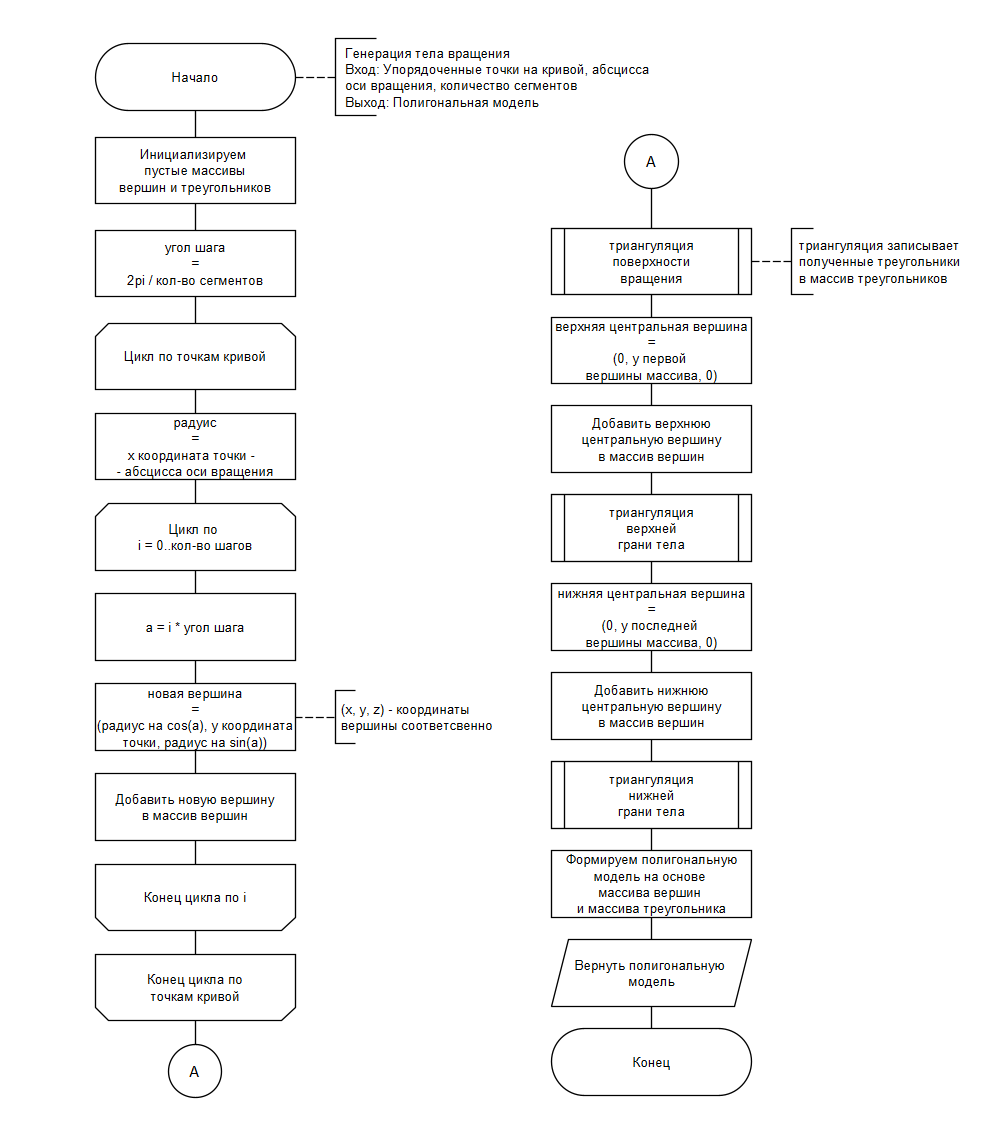
\includegraphics[width=1\linewidth]{images/diograms/gen_body.png}
    \caption{Алгоритм генерации тела вращения}
    \label{fig:gen_body}
\end{figure}

\section{Общий алгоритм построения изображения}

Алгоритм генерации изображения представлен на рисунке~\ref{fig:gen_alg}. 

\textbf{Вход:} тело вращения и источник света, переведенные в пространство камеры. 

\textbf{Выход:} изображение трехмерной сцены в виде матрицы пикселей.

\begin{figure}[H]
    \centering
    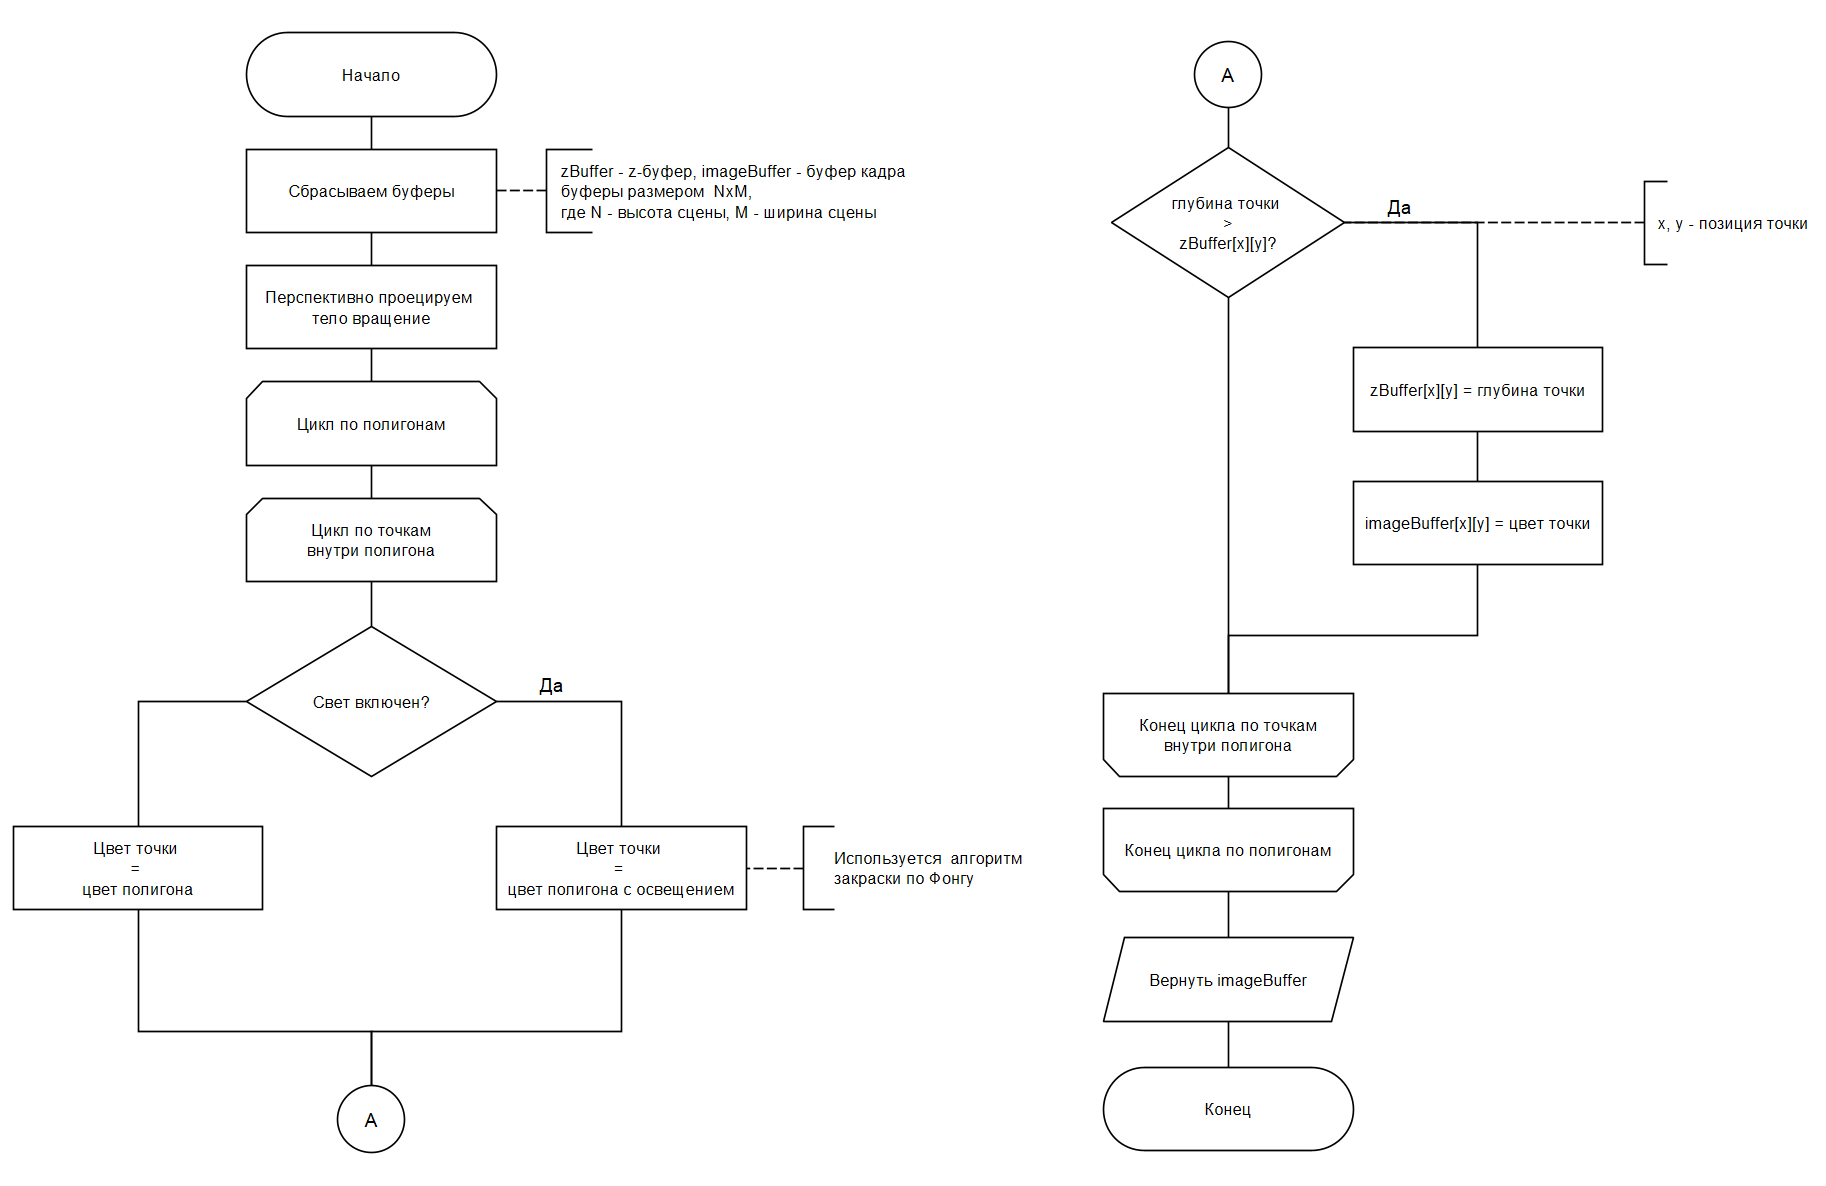
\includegraphics[width=1\linewidth]{images/diograms/gen_alg.png}
    \caption{Общий алгоритм построения изображения}
    \label{fig:gen_alg}
\end{figure}

\section{Описание алгоритма Z-буфера}

Z-буфер (или глубинный буфер) — это метод, используемый для скрытия невидимых поверхностей и определения, какие пиксели объекта должны отображаться на экране при наложении трёхмерных объектов. Z-буфер работает на основе хранения значений глубины (Z-координат) для каждого пикселя сцены.

\begin{enumerate}
    \item Буфер кадра $c_{buf}$ заполняется фоновым цветом, z-буфер $z_{buf}$ заполняется $-\infty$.
    \item Для каждого полигона сцены:
    \begin{itemize}
        \item[---] вычисляется глубина $z(x,y)$ для каждого пикселя полигона;
        \item[---] Сравнивается глубина пикселя со значением глубины в z-буфере. Если $z(x,y) > z_{buf}(x,y)$, то $z_{buf}(x,y) = z(x,y)$ и $c_{buf} = colour$.
    \end{itemize}
    \item Вернуть буфер кадра.
\end{enumerate}

Схема алгоритма z-буфера представлена на рисунке~\ref{fig:z_buf}.

\begin{figure}[H]
    \centering
    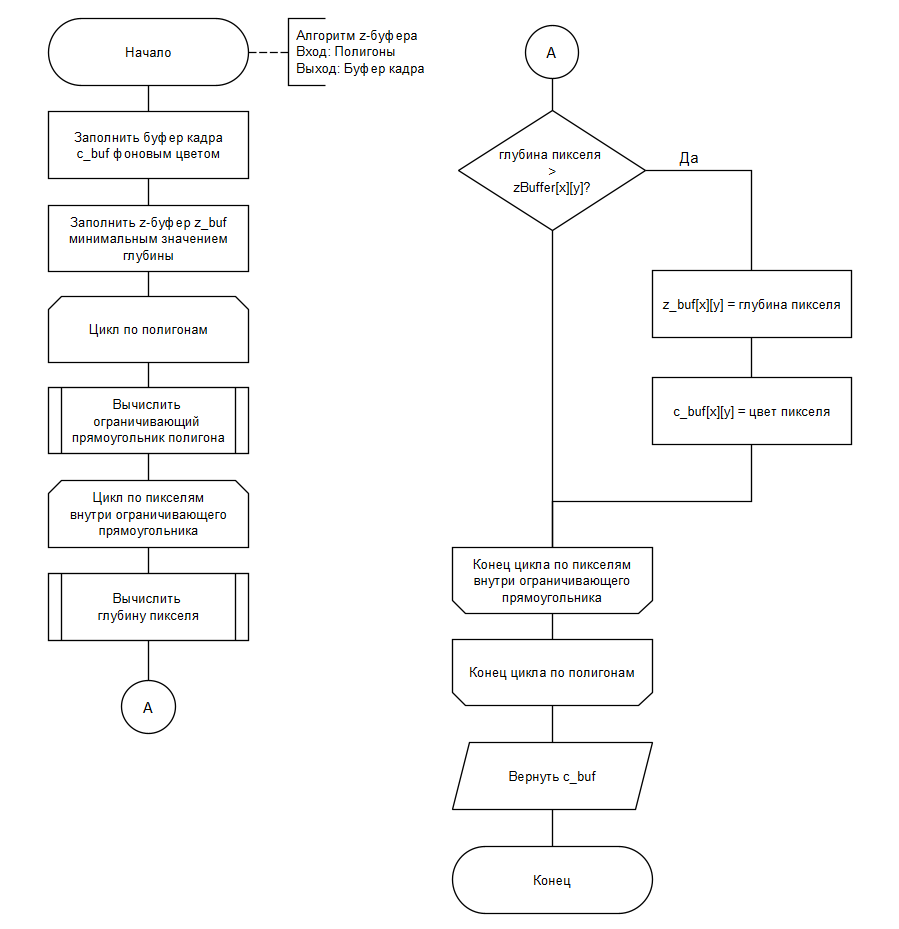
\includegraphics[width=1\linewidth]{images/diograms/z_buf.png}
    \caption{Схема алгоритма z-буфера}
    \label{fig:z_buf}
\end{figure}

\paragraph*{ВЫВОД} ${}$ \\

В данном разделе были представлены требования к программному обеспечению, рассмотрены структуры данных и алгоритмы, выбранные для построения сцены.
